\documentclass[9pt]{beamer}
\usepackage[UTF8]{ctex}

% we are running LaTeX, not pdflatex


\usepackage{xcolor}
\usepackage{layouts}
\usepackage{minted}
\usepackage[most]{tcolorbox}
\tcbuselibrary{minted}
\usepackage{booktabs}
\usepackage{outlines}
\usepackage{hyperref}
\usepackage{graphicx}
\beamertemplatenavigationsymbolsempty
\usepackage{fontspec}
\setmonofont{Fira Code}[Contextuals=Alternate]


\AtBeginSection[]{
  \begin{frame}
  \tableofcontents[currentsection, hideothersubsections]
  \end{frame}
}

% color
\definecolor{coreFontMain}{RGB}{26,26,26}
\definecolor{coreFontSub}{RGB}{106,106,106}
\definecolor{coreBackgroundLight}{RGB}{230,230,230}
\definecolor{coreBackground}{RGB}{255,255,255}

% heading
\newlength{\headerheight}
\setlength{\headerheight}{0.094\paperheight}


\setbeamerfont{frametitle}{size=\fontsize{12}{14.4}}
\setbeamertemplate{frametitle}
{%
\nointerlineskip
\begin{beamercolorbox}[wd=\paperwidth,left,sep=0pt]{}
\begin{tcolorbox}[enhanced,frame hidden, 
    borderline south={0.5pt}{0pt}{coreFontSub},
    colback=coreBackground, coltext=coreFontSub,height=\headerheight,notitle,left*=0.05\paperwidth,boxsep=0pt,bottom=0pt,halign=left,valign=bottom,before skip=0pt,after skip=0pt, before upper=\strut]
    \usebeamercolor{frametitle}\insertframetitle
\end{tcolorbox}
\end{beamercolorbox}
}


% footer
\newlength{\footerheight}
\setlength{\footerheight}{0.04\paperheight}
\setbeamercolor{footer}{bg=coreBackgroundLight, fg=coreFontMain}

\setbeamertemplate{footline}
{%
\begin{beamercolorbox}[sep=0pt,wd=\paperwidth,center]{footer}
\begin{minipage}[c][\footerheight]{\textwidth}
    \centering
    \insertframenumber/\inserttotalframenumber
\end{minipage}
\end{beamercolorbox}
}



% Title Page

% header
\newlength{\titleheaderheight}
\setlength{\titleheaderheight}{0.0666667\paperheight}
\setbeamercolor{header}{bg=coreBackgroundLight}

%% logo
\newlength{\logoheight}
\setlength{\logoheight}{0.297\paperheight}

%% title
\setbeamercolor{title}{fg=coreFontMain}
\setbeamerfont{title}{size=\fontsize{18.14}{21.768}}
\newlength{\titleheight}
\setlength{\titleheight}{0.19\paperheight}


%% meta
\newlength{\metaheight}
\setlength{\metaheight}{0.21\paperheight}
\setbeamercolor{meta}{fg=coreFontSub}
\setbeamerfont{meta}{size=\fontsize{9.07}{10.884}}

%% contact
\newlength{\contactheight}
\setlength{\contactheight}{0.193333\paperheight}



\setbeamertemplate{title page}{
\nointerlineskip
\begin{beamercolorbox}[wd=\paperwidth,ht=\titleheaderheight]{header}
\end{beamercolorbox}
\nointerlineskip
\begin{beamercolorbox}[wd=\paperwidth,ht=\logoheight]{}
\end{beamercolorbox}
\nointerlineskip
\begin{tcolorbox}[enhanced,frame hidden, borderline south={0.5pt}{0pt}{coreFontMain}, colback=coreBackground,height=\titleheight,boxsep=0pt,bottom=20pt,notitle,halign=flush center,valign=center,before skip=0pt,after skip=0pt, coltext=coreFontMain]
\usebeamercolor{title}
\usebeamerfont{title}\inserttitle

\end{tcolorbox}

\usebeamercolor[fg]{meta}{
\begin{minipage}[c][\metaheight]{\textwidth}
    \centering
    \insertauthor \linebreak
    \insertinstitute \linebreak
    \insertdate
\end{minipage}
}


\begin{tcolorbox}[enhanced,frame hidden, colback=coreBackground,height=\contactheight,notitle,halign=flush center,valign=top,before skip=0pt,after skip=0pt,top=-5pt]
\begin{tabular}{ccc}
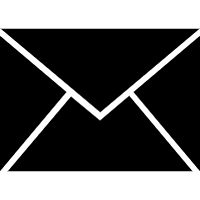
\includegraphics[height=3mm]{bohanbeamerstyle/figures/mail.png} & 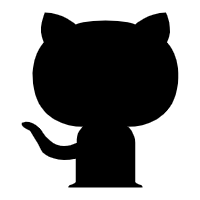
\includegraphics[height=3mm]{bohanbeamerstyle/figures/github.png} &
\includegraphics[height=3mm]{bohanbeamerstyle/figures/Twitter.png}
\end{tabular}

\end{tcolorbox}




\begin{beamercolorbox}[sep=2pt,center,wd=\paperwidth,ht=\footerheight]{footer}
\tiny
\insertframenumber/\inserttotalframenumber
\end{beamercolorbox}
\nointerlineskip
}


% 
\setbeamercolor{normal text}{bg=coreBackground,fg=coreFontMain}

% itemize
\setbeamertemplate{itemize items}[circle]

\setlength{\leftmarginii}{10pt}
\setbeamercolor{itemize item}{fg=coreFontMain}
\setbeamercolor{itemize subitem}{fg=coreFontMain}
\setbeamercolor{itemize subsubitem}{fg=coreFontMain}



% code

\newtcblisting{codebox}[2]{listing only, title={#2}, minted language={#1}, minted style=xcode, minted options={fontsize=\fontsize{8}{9.6}, fontfamily=tt}, left=3mm}

\title{Python入门(五)}
\author{张博涵}
\institute{北京航空航天大学}
\date{\today}

\begin{document}

\begin{frame}[plain]
\maketitle
\end{frame}

\begin{frame}
    \frametitle{Contents}

    \tableofcontents

\end{frame}

\section{类与对象}

\begin{frame}
    \frametitle{类与对象 - Class \& Object}
    \begin{block}{类 - Class}
    \begin{itemize}
        \item 类(Class)是数据类型(Data Type)在Python中的实现,其他语言中类似的名称有Struct(结构体)
        \item Class一般指向一类事物,例如人、一类算法、一类比赛。
        \item Class通常由两方面组成:属性(attributes)以及方法(methods)
        \item 属性通常用于存放数据(Data)或状态(state),例如人的身高体重、算法的初始值与输入、比赛的对战双方。状态如人的年龄、算法的运行阶段、比赛是否开始。
        \item 方法为对数据类型进行的某种操作(action),进行操作后通常会使得存储的数据或状态发生改变。例如人``过生日''会使得年龄+1,算法``开始''通常会伴随着某些初始化,比赛``结束''可能伴随着成绩变化。
    \end{itemize}
    \end{block}

\end{frame}

\begin{frame}
    \frametitle{类与对象 - Class \& Object}

    \begin{block}{对象 - Object}
    \begin{itemize}
        \item 对象是类的实例(instances),它通常指向属于这种数据类型的某个具体事物,例如具体的人、某个具体的算法、某场比赛。
        \item 对象的属性有具体的值,可以获取或通过方法进行修改。
    \end{itemize}

    \end{block}
    \begin{block}{面向对象编程}

        \begin{itemize}
        \item  围绕类、对象、方法、属性等进行程序构建的编程范式被称为``面向对象编程''(Object Oriented Programming, OOP),Python对OOP有非常完整的支持,OOP也是Python中应用最广泛的编程范式。
        \item Python还支持OOP的其他特性如继承(inheritance)
        \end{itemize}

        
    \end{block}


    

\end{frame}


\begin{frame}[fragile]
    \frametitle{Class 定义}

\begin{codebox}{python}{Class}
class Person(object):
    def __init__(self, name, age = 18):
        self.name = name
        self.age = age
    def say(self, stuff):
        return self.name + ' says: ' + stuff
    def birthday(self):
        self.age += 1
        return self.age
    def __str__(self):
        return self.name
\end{codebox}

\pause
\begin{itemize}
    \item \mintinline{python}{(object)}表示继承`object'对象,如果继承对象是`object',可以不写。
    \item 在\mintinline{python}{class}代码块内的定义的函数,主要包含\alert{对象方法}和\alert{类方法}。
    \item \mintinline{python}{__init__}方法称为类型的构造器(constructor),在将类实例化为对象时调用。
    \item \mintinline{python}{self}指向实例化对象,必须作为对象方法的第一个参数,代表其是一个对象方法。
\end{itemize}
    

\end{frame}


\begin{frame}[fragile]
    \frametitle{Class 定义}

\begin{codebox}{python}{Class}
class Person(object):
    def __init__(self, name, age = 18):
        self.name = name
        self.age = age
    def say(self, stuff):
        return self.name + ' says: ' + stuff
    def birthday(self):
        self.age = self.age + 1
        return self.age
    def __str__(self):
        return self.name
\end{codebox}

\pause
\begin{itemize}
    \item \mintinline{python}{name}, \mintinline{python}{age}为实例化对象的属性(attributes),分别存储某个人的姓名和年龄。
    \item 在类的定义以及类方法内部,可以通过\mintinline{python}{self.xxx}访问对象属性或者方法。
    \item 在方法内部生成的\mintinline{python}{self.}开头的变量都可以称为对象的属性,而在方法外部,类的内部生成的变量称为类的属性
\end{itemize}
    

\end{frame}


\begin{frame}[fragile]
\frametitle{类的实例化:对象}

\begin{codebox}{python}{Object}
bohan = Person(name='张博涵', age=24)
bohan.name # 张博涵(访问对象属性)
bohan.age # 24(访问对象属性)
bohan.type # animal(访问类属性)
bohan.birthday() # 25(调用对象的方法)
bohan.say("Hello") # 张博涵 says: Hello(调用对象的方法)
\end{codebox}
    
\begin{itemize}
    \item 类似于函数调用的方式调用类名,会调用类的\mintinline{python}{__init__}方法并传入除\mintinline{python}{self}以外的参数来创建类的对象。
    \item 对象可以通过\mintinline{python}{object_name.xxx}来访问自身的属性(即定义中\mintinline{python}{self.xxx}创建的属性),也可以访问类属性,同样通过这种方式来调用方法。
    \item 一般情况下属性可以对属性直接修改,但不建议这么做,例如\mintinline{python}{bohan.age = 26}
    \item 需要格外注意的是,类(Class)和对象(Object)是非常不同的两个概念,一定要注意区分。Object是Class的实例(instance)。
\end{itemize}

\end{frame}


\begin{frame}
    \frametitle{深入区分类与对象}

    \begin{block}{类的命名空间(namespace)}

        \begin{itemize}
            \item 类的命名空间在类定义时即创建,例如之前的\mintinline{Python}{class Person:},其中包括类属性(例如\mintinline{python}{type})以及所有函数(例如\mintinline{python}{__init__}, \mintinline{python}{ask})
            \item 也包括一些隐藏属性,例如\mintinline{python}{__doc__, __base__, __dict__}
            \item 类型的属性可以通过重新赋值来改变,例如: \mintinline{python}{Person.type = 'animals'}
        \end{itemize}
        
    \end{block}

    \begin{block}{对象的命名空间}
        \begin{itemize}
            \item 在实例化创建对象后,创建的对象拥有属于自己的命名空间。
            \item 对象定义中的所有\mintinline{python}{self}函数转换为对象的方法(e.g., \mintinline{python}{bohan.ask()}),实际上,在调用方法时,将对象作为函数的第一个参数,即\mintinline{python}{bohan.ask(stuff) = Person.ask(bohan, stuff)}
            \item 通过构造器或其他方法创建了对象的属性(e.g.\mintinline{python}{bohan.name},这些属性有时也被称为数据属性)
            \item 对象可以直接访问类属性,但不可修改它,但若对象有某个属性的名字与类属性名字相同,则以对象的属性为准。
        \end{itemize}
    \end{block}

\end{frame}


\section{继承 - Inheritance}


\begin{frame}[fragile]
    \frametitle{继承 - Inheritance}

    \begin{codebox}{python}{Syntax}
class DerivedClassName(BaseClassName):
    <statement-1>
    .
    .
    .
    <statement-N>
class DerivedClassName(moduleName.BaseClassName):
\end{codebox}

\begin{itemize}
    \item \mintinline{python}{DerivedClassName}\alert{继承}了\mintinline{python}{BaseClassName}
    \item 可以将\mintinline{python}{DerivedClassName}理解为\mintinline{python}{BaseClassName}的一个子空间,当访问\mintinline{python}{BaseClassName}的某个函数或属性时,若在当前空间中没有发现,则会在他的父空间即\mintinline{python}{BaseClassName}中寻找,同理\mintinline{python}{BaseClassName}也会从自身的父空间中寻找。
    \item 例如之前提到的\mintinline{python}{__doc__}、\mintinline{python}{__base__}等虽然没有定义,但该对象继承了\mintinline{python}{object}对象。
    \item 继承类的实例化和之前讲的一致。
\end{itemize}

\end{frame}

\begin{frame}
    \frametitle{继承的其他特性}

    \begin{itemize}
        \item 重载(overload)指在子类中创建一个和父类相同名字的方法\mintinline{python}{xxx},根据命名空间规则,子类对象会访问该方法\mintinline{python}{DerivedClassName.xxx}而不是父类的该方法\mintinline{python}{BaseClassName.xxx}。
        \item 在\mintinline{python}{DerivedClassName}的对象方法内部可以通过\mintinline{python}{super().xxx}访问父类的\mintinline{python}{xxx}方法,这在想要扩展父类的方法而不是直接替代父类方法时很有用,在\mintinline{python}{__init__}中应用广泛。
        \item \mintinline{python}{isinstance(obj, cls1)}判断对象\mintinline{python}{obj}是否是\mintinline{python}{cls1}类型或它的子类型。
        \item \mintinline{python}{isubclass(cls1, cls2)},判断\mintinline{python}{cls1}是否是\mintinline{python}{cls2}的子类型。
        \item Python还支持 Multiple Inheritance(多类继承)、classmethod(类方法)等其他特性。
    \end{itemize}
    
\end{frame}

\section{特殊类方法}

\begin{frame}
    \frametitle{Iterator - 可迭代对象}

    从具体实现上来看,需要支持以下方法来实现类的迭代器:

    \begin{itemize}
        \item 实现\mintinline{python}{__iter__()},该方法需要返回一个新的对象,这个对象的类应该具有\alert{可迭代特性}。
        \item 具体来说,这个类型需要实现\mintinline{python}{__next__()}方法,该方法返回一个数值,当迭代到最后一个值时,报出\mintinline{python}{StopIteration}错误。
    \end{itemize}

    \begin{block}{生成器 - Generator}
        \begin{itemize}
            \item 生成器是快速生成一个Iterator的一类函数。
            \item 这类函数在返回时不用\mintinline{python}{return}关键字,而用\mintinline{python}{yield}关键字
            \item 调用这种函数会返回一个\mintinline{python}{generator}对象,该对象实现了\mintinline{python}{__next__()}方法
        \end{itemize}
    \end{block}

\end{frame}

\begin{frame}
    \frametitle{回调/分发: callback/dispatch}

    \begin{itemize}
        \item 在Python中,在调用一些内置函数,例如\mintinline{python}{str(x)}, \mintinline{python}{bool(x)}, \mintinline{python}{len(x)}, \mintinline{python}{class(x)}时,实际上是调用了\mintinline{python}{x.__xxx__()}方法,这种行为称为callback或者dispatch
        \item 前面的\mintinline{python}{__next__}以及\mintinline{python}{__iter__}则可以分别通过\mintinline{python}{next()}以及\mintinline{python}{iter()}函数去调用。
    \end{itemize}

\end{frame}

\section{作业}

\begin{frame}
    \frametitle{作业}

    实现一个比赛类,它包含以下属性:

    \begin{itemize}
        \item 对战双方
        \item 比赛比分
        \item 比赛状态
    \end{itemize}

    以下如下方法:

    \begin{itemize}
        \item 比赛开始,可以开始计分
        \item 得分方法,当某对得分时,其分数加1,若比赛已结束或未开始,则什么都不做,并提示用户。
        \item 比赛结束方法,输出最终比分并输出胜者。
        \item \mintinline{python}{__str__}方法,当输入这场比赛时,输出对战双方、目前比分,比赛状态。
    \end{itemize}

\end{frame}

\end{document}